 % PoR algorithms

 \begin{algorithm}
\caption{Vanilla chain-weight algorithm (typical of traditional blockchains).}\label{alg:vanilla-bw}
\begin{algorithmic}
\Procedure{ChainWeight}{$blocks$, $state$}\Comment{The weight of a chain}
  \If {length($blocks$) == 0}
    \State \Return{0}
  \EndIf
  \State \Return{\Call{BlockWeight}{head($blocks$), $state$} + \Call{ChainWeight}{tail($blocks$), $state$}}
\EndProcedure
\\
\Procedure{BlockWeight}{$block$, $state$} \Comment{The weight of an individual block}
  \State \Return{\Call{LocalBlockWeight}{$block$, $state$}} \Comment{NB: defined by the consensus method}
\EndProcedure
\end{algorithmic}
\end{algorithm}

 
\begin{algorithm}
\caption{Modified chain-weight algorithm to factor in reflections.}
\label{alg:refl-1-bw}
\begin{algorithmic}
\Procedure{ChainWeight}{$blocks$, $state$} \Comment{The weight of a blockchain}
  \If {length($blocks$) == 0}
    \State \Return{0}
  \EndIf
  \State \Return{\Call{BlockWeight}{head($blocks$), $state$} + \Call{ChainWeight}{tail($blocks$), $state$}}
\EndProcedure
\\
\Procedure{BlockWeight}{$block$, $state$}
  \State $W_l \gets$ \Call{LocalBlockWeight}{$block$} \Comment{Weight due to work done producing $block$}
  \State $W_r \gets$ \Call{ReflectedBlockWeight}{$block$, $state$} \Comment{Weight added via reflection}
  \State \Return{$W_l + W_r$}
\EndProcedure
\\
\Procedure{ReflectedBlockWeight}{$L_i$, $state$}
  \State $w\gets 0$ \Comment{Sum of weights}
  \State $R_{\text{blocks}} \gets$ \Call{ReflectingRBlocks}{$state$} \Comment{Chain R blocks that reflect the local chain}
  \For{$R_i$ in $R_{\text{blocks}}$}
    \State RCHs $\gets$ \Call{ReflectedChainHeads}{$R_i$, $state$} \Comment{Local blocks reflected by $R_i$}
    \If {$L_i$ in RCHs}
      \State $w \gets w\;+$ \Call{WeightOf}{$R_i$, $state$} \Comment{NB: network specific, e.g., \autoref{alg:weightof-1}}
    \EndIf
  \EndFor
  \State \Return{w}
\EndProcedure
\end{algorithmic}
\end{algorithm}

 \begin{algorithm}
\caption{A simplistic \textsc{WeightOf} for networks of a single root token with equal block frequencies}\label{alg:weightof-1}
\begin{algorithmic}
\Procedure{WeightOf}{$B_i, state$} \Comment{The weight of a block normalized to coins}
    \State $t \gets$ \Call{BlockTimestamp}{$B_i$}
    \State $C \gets$ \Call{ChainOf}{$B_i$, $state$} \Comment{Either the local or a reflecting chain}
    \State $C_r \gets$ \Call{BlockRewardOfChainAt}{$C$, $t$, $state$} \Comment{Block reward of $C$ at $t$}
    \State \Return{$C_r$}
\EndProcedure
\end{algorithmic}
\end{algorithm}

 \begin{algorithm}
\caption{A \textsc{WeightOf} function for one-way PoR between chains with different root tokens}
\label{alg:weightof-dex-one-way}
\begin{algorithmic}
\Procedure{WeightOf}{$B_i$, $state$} \Comment{Convert reflecting weight to local via a DEX}
    \State $t \gets$ \Call{BlockTimestamp}{$B_i$}
    \State $C \gets$ \Call{ChainOf}{$B_i$, $state$}
    \State $C_r \gets$ \Call{BlockRewardOfChainAt}{$C$, $t$, $state$} \Comment{Block reward of $C$ at $t$}
    \State $C_f \gets$ \Call{BlockFrequencyOfChainAt}{$C$, $t$, $state$}
    \State $L_d \gets$ \Call{DifficultyOfLocalAt}{$t$, $state$}
    \State $L_f \gets$ \Call{BlockFrequencyOfLocalAt}{$t$, $state$}
    \State $L_r \gets$ \Call{BlockRewardOfLocalAt}{$t$, $state$}
    \State $X_{C\rightarrow L} \gets$ \Call{GetLocalDexRateFromAt}{$C$, $t$, $state$}
    % \State $w \gets$ \Call{$\text{ConvDEX}_{R\rightarrow L}$}{$L_d$, $L_f$, $L_r$, $C_f$, $C_r$, $X_{C\rightarrow L}$}
    \State \Return{\Call{$\text{ConvDEX}_{R\rightarrow L}$}{$L_d$, $L_f$, $L_r$, $C_f$, $C_r$, $X_{C\rightarrow L}$}}
\EndProcedure
\\
\Procedure{$\text{ConvDEX}_{R\rightarrow L}$}{$L_d$, $L_f$, $L_r$, $R_f$, $R_r$, $X_{R\rightarrow L}$} \Comment{Returns L-hashes/L-block}
    \State \Return{$(L_d \div L_r) \cdot X_{R\rightarrow L} \cdot R_r \cdot (R_f \div L_f)$} \Comment{See \autoref{eq:por-conv-dex}}
\EndProcedure
\end{algorithmic}
\end{algorithm}


\begin{algorithm}
\caption{A \textsc{WeightOf} function for PoR between chains with a different root token and equal block frequencies}
\label{alg:weightof-dex}
\begin{algorithmic}
\Procedure{WeightOf}{$B_i, state$} \Comment{The weight of a block normalized to coins}
    \State $t \gets$ \Call{BlockTimestamp}{$B_i$}
    \State $C \gets$ \Call{ChainOf}{$B_i$, $state$}
    \State $C_r \gets$ \Call{BlockRewardOfChainAt}{$C$, $t$, $state$} \Comment{Block reward of $C$ at $t$}
    % \State $C_f \gets$ \Call{BlockFrequencyOfChain}{$C$} \Comment{Block production Hz of $C$}
    \State $X_{C\rightarrow L} \gets$ \Call{ExchangeRateOfCoinToLocalAt}{$C$, $t$, $state$}
    \State \Return{$C_r \cdot X_{C\rightarrow L}$}
\EndProcedure
\end{algorithmic}
\end{algorithm}

 \begin{algorithm}
\caption{Many-chain ReflectedBlockWeight}
\label{alg:por-reflected-block-weight}
\begin{algorithmic}
\Procedure{ReflectedBlockWeight}{$block, state$}
  \State $w\gets 0$ \Comment{Sum of weights}
  \For{$C$ in \Call{AllReflectingChains}{$state$}}
    \State $w_C \gets 0$ \Comment{Sum of weights for this chain}
    \State $n \gets 0$
    \State $blocks \gets$ \Call{Reflectingb}{$C$, $state$} \Comment{Reflecting blocks from $C$}
    \For{$B_i$ in $blocks$}
      \State RCHs $\gets$ \Call{ReflectedChainHeads}{$B_i$, $state$} \Comment{Local blocks reflected by $B_i$}
      \If {$block$ in RCHs}
        \State $n \gets n + 1$
        \State $s_C \gets s_C \; +$ \Call{WeightOf}{$B_i$, $state$}
      \EndIf
    \EndFor
    \State $\text{weightMod} \gets $ \Call{CapWorkOf}{$C$, $n$, $state$}
    \State $s \gets s + s_C \cdot \text{weightMod}$
  \EndFor
  \State \Return{$s$}
\EndProcedure \Comment{This is an inefficient method and would not be used in production.}
\\
\Procedure{CapWorkOf}{$C$, $n$, $state$} \Comment{A simplistic method for capping work}
  \If {$n \le 0$}
    \State \Return{0}
  \EndIf
  \State $B_f \gets $ \Call{BlockFrequencySelf}{$state$}
  \State $C_f \gets $ \Call{BlockFrequencyOfChain}{$C$, $state$}
  \State $e \gets C_f \div B_f$ \Comment{Expected blocks from $C$}
  \State \Return{min(1, $e \div n$)} \Comment{This caps the contribution of $C_i$ per block}
\EndProcedure
\end{algorithmic}
\end{algorithm}

 \begin{comment}
\begin{algorithm}
\caption{Simplex PoR adjustments}
\label{alg:por-simplex}
\begin{algorithmic}
\Procedure{WeightOf}{$B, state$}
    \State \todo{write por-simplex WeightOf algorithm}
\EndProcedure
% \Procedure{ReflectedBlockWeight}{$block, state$}
% \State $s\gets 0$
% \For{$C_i$ in \Call{AllReflectingChains}{$state$}}
%     \State $Blocks_{i} \gets$ \Call{ReflectingBlocks}{$C_i$, $state$} \Comment{Reflecting blocks from $C_i$}
%     \For{$B_{i,j}$ in $Blocks_{i}$}
%         \State RCHs $\gets$ \Call{ReflectedChainHeads}{$B_{i,j}$, $state$} \Comment{Local blocks reflected by $B_{i,j}$}
%         \If {$block$ in RCHs}
%             \State $s\gets s \; +$ \Call{WeightOf}{$B_{i,j}$, $state$}
%         \EndIf
%     \EndFor
% \EndFor
% \State \Return{s}
% \EndProcedure \Comment{This is an inefficient method and would not be used in production.}
\end{algorithmic}
\end{algorithm}
\end{comment}


 % one way PoR

 \begin{figure}
     \centering
     \includegraphics[width=.8\linewidth]{../ut/diags/pow_refl_step3_ab_sag}
     \caption{The time-evolution of, and relationship between, two separate blockchains, A and B, where Chain A is using Chain B for PoR.}
     \label{fig:por-step3}
 \end{figure}

 % mutual reflection

 \begin{figure}
     \centering
     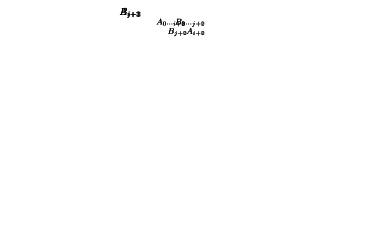
\includegraphics[width=.8\linewidth]{../ut/diags/pow_refl_step5_sag}
     \caption{Relationships between and time-evolution of two blockchains that are mutually reflecting one another.}
     \label{fig:por-step5}
 \end{figure}

 % simplexes

 \begin{figure}
    \begin{subfigure}[t]{.31\linewidth}
        \vskip 0pt
        \centering
        \includegraphics[height=.95\linewidth]{simplex_2_sag}
        \caption{\raggedright Proof of Reflection between 2 blockchains. A 1-simplex. The most basic non-trivial simplex.}
        \label{fig:simplex-2-d1}
    \end{subfigure}%%
    \hfill
    \begin{subfigure}[t]{.31\linewidth}
        \vskip 0pt
        \centering
        \includegraphics[height=.95\linewidth]{simplex_7_sag}
        \caption{\raggedright Proof of Reflection between 7 blockchains; a 7-chain simplex; a 6-simplex.}
        \label{fig:simplex-7-d1}
    \end{subfigure}%%
    \hfill
    \begin{subfigure}[t]{.31\linewidth}
        \vskip 0pt
        \centering
        \includegraphics[height=.95\linewidth]{simplex_17_sag}
        \caption{A 17-chain simplex; a 16-simplex. It has 136 unique mutual reflections in total.}
        \label{fig:simplex-17-d1}
    \end{subfigure}
    \caption{Simplexes of increasing capacity. Vertices are simplex-chains. Edges are the reflections between simplex-chains.}
    \label{fig:simplexes}
 \end{figure}
